\section{Effect of transformation on model}
From literature review we postulate that small changes to input image should not affect the prediction model. In this thesis we investigate the effect of the identified metamorphic properties have on the accuracy of model. For each machine learning algorithms generated ten models . For each metamorphic property identified in section X we look how it affects . We calculated the following metrics to evaluate the affect of metamophic relations on deep-learning algorithm. To tackle the non-deterministic nature of training a neural network model, we ran each of the above experiment ten times and calculated average.
\subsection{Overall Accuracy or true positive}
    Accuracy is defined as the number of correct predictions made by the model with respect to the total number of predictions made.
\subsection{Digit-by Accuracy or true positive for each digit}
    We analyze each digit and 
\subsection{Misclassification of digits}
    In order to see how each digit is affected by changes in  mp. For each digit 0-9 we calculated the number of correct predictions made by the model as compared to total number of .
\subsection{Robustness}
    
    
\clearpage
% \section{Overall Accuracy}
The 
    \begin{figure}[!htb]
        \begin{center}
          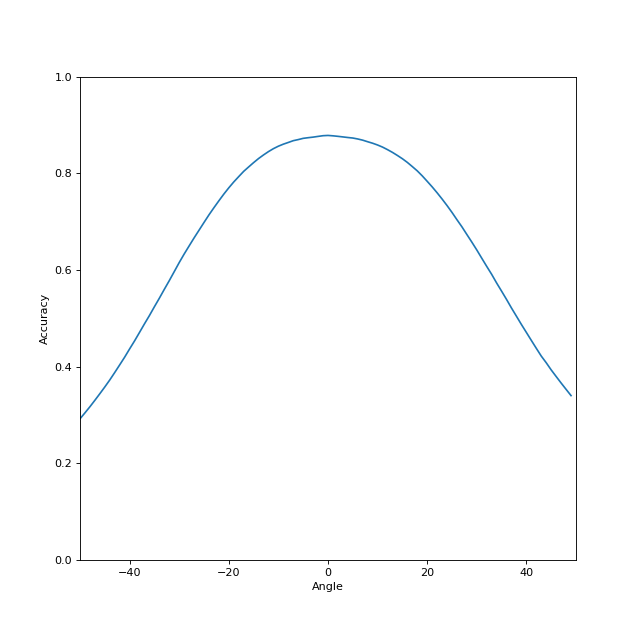
\includegraphics[scale=0.6]{chapters/results/CNN/Rotate/acc.png}
          \caption{Overall accuracy for metamorphic relation rotation.}
          \label{fig:Rotate 1}
        \end{center}
    \end{figure}
    
\clearpage
    \begin{figure}[!htb]
    \centering
      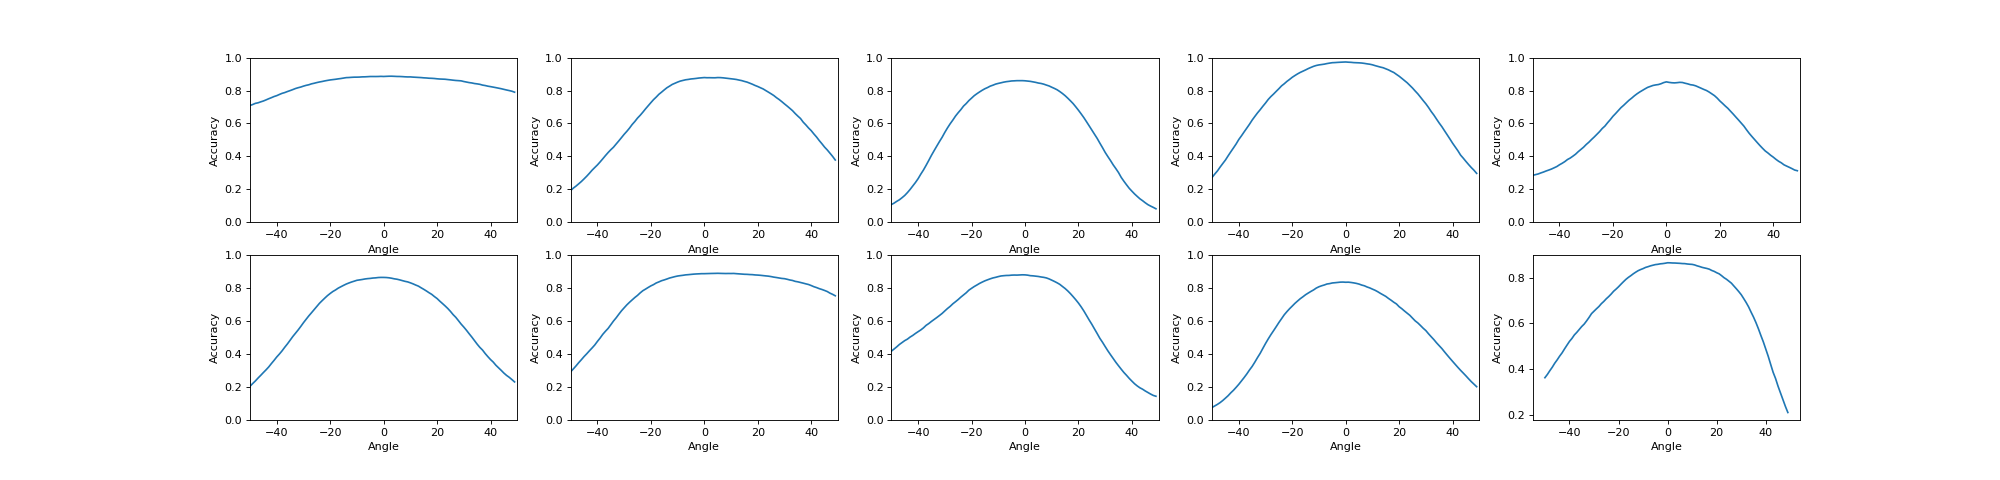
\includegraphics[width=\linewidth]{chapters/results/CNN/Rotate/accAll.png}
      \caption{Accuracy of each digit.}
      \label{fig: Shading}
    \end{figure}
        
\clearpage
\begin{figure}[htb!]
    \centering
    \begin{subfigure}[b]{\textwidth}
        \centering
        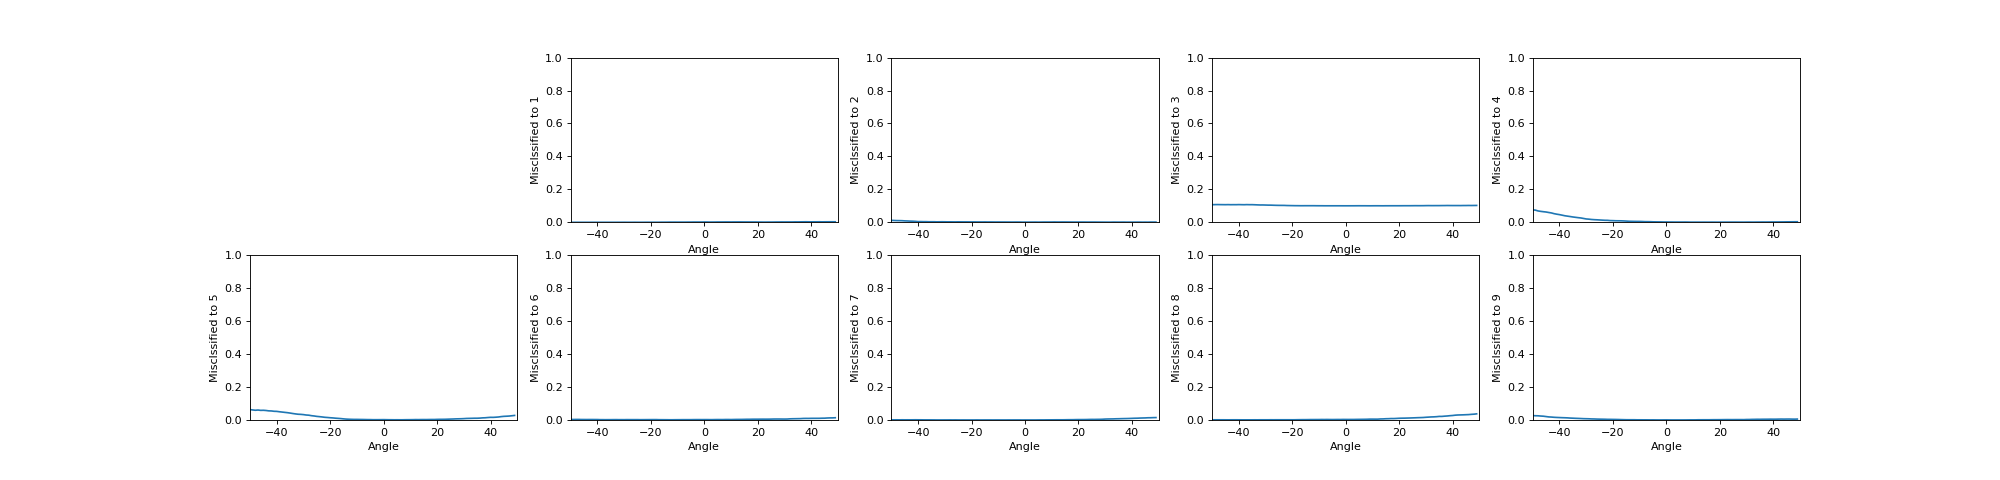
\includegraphics[width=\textwidth]{chapters/results/CNN/Rotate/acc1.png}
        \caption{Misclassification of Digit 0}
        \label{fig:Rotate-misclass0}
    \end{subfigure}
    \begin{subfigure}[b]{\textwidth}
        \centering
        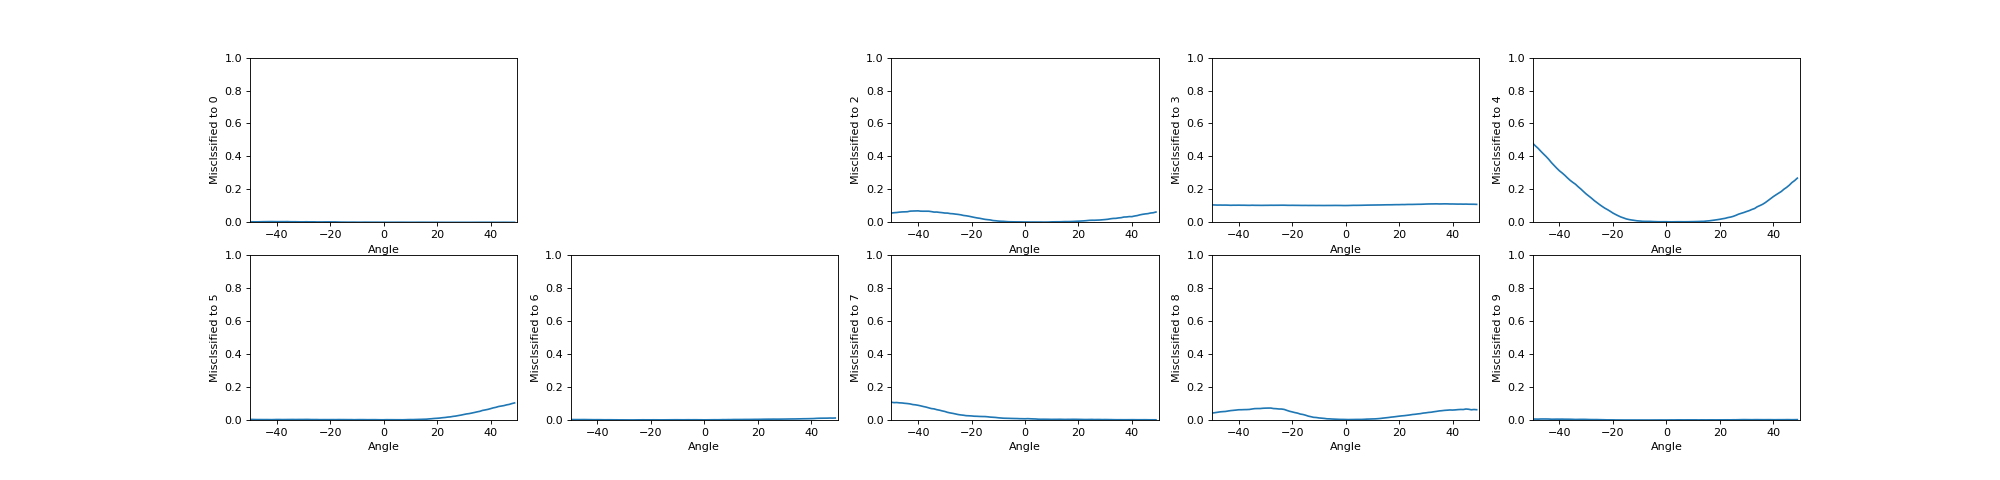
\includegraphics[width=\textwidth]{chapters/results/CNN/Rotate/acc2.png}
        \caption{Misclassification of Digit 1}
        \label{fig:Rotate-misclass0}
    \end{subfigure}
    \begin{subfigure}[b]{\textwidth}
        \centering
        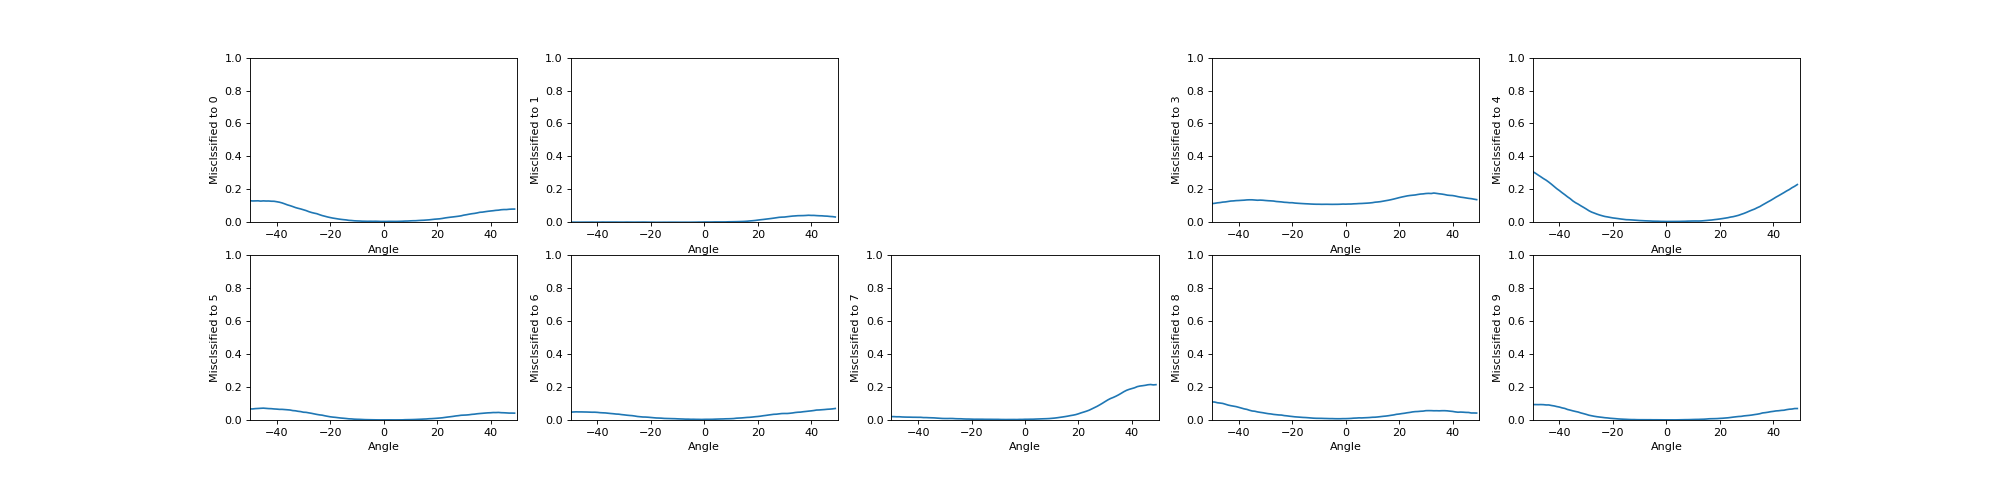
\includegraphics[width=\textwidth]{chapters/results/CNN/Rotate/acc3.png}
        \caption{Misclassification of Digit 2}
        \label{fig:Rotate-misclass0}
    \end{subfigure}
    \begin{subfigure}[b]{\textwidth}
        \centering
        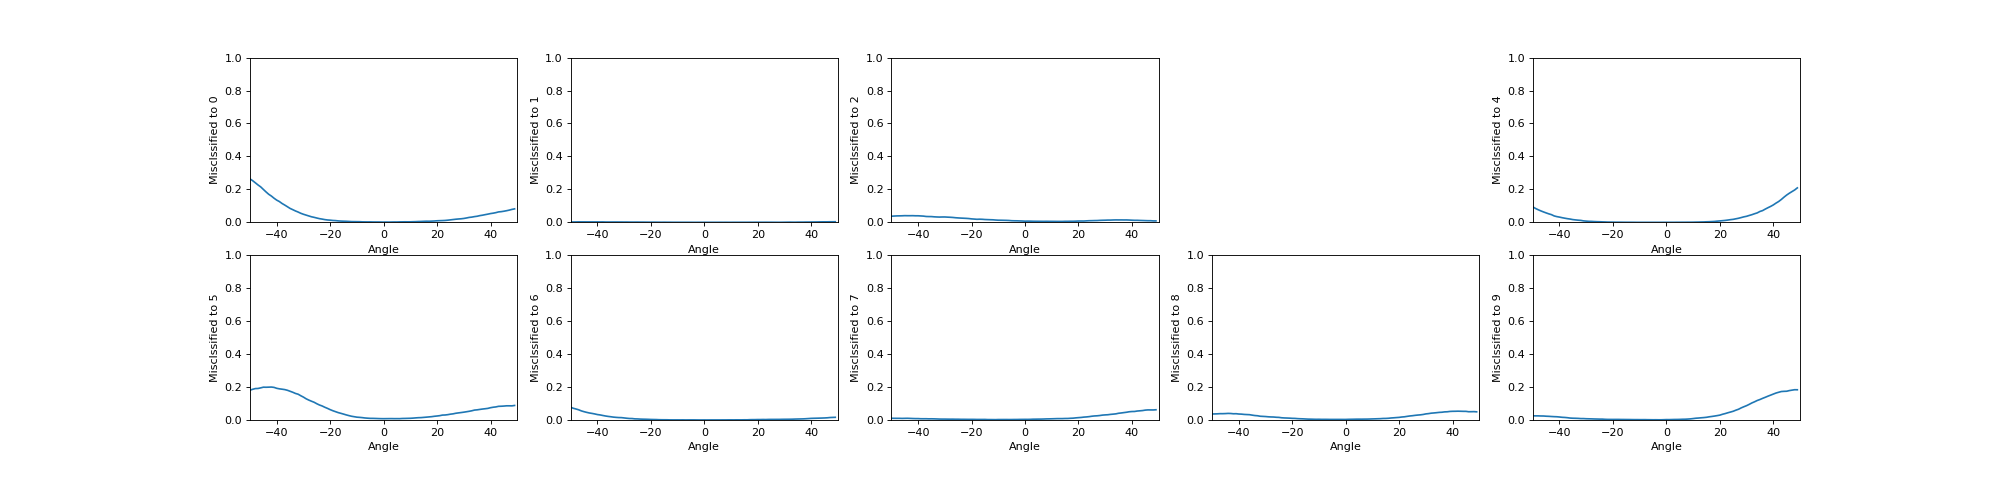
\includegraphics[width=\textwidth]{chapters/results/CNN/Rotate/acc4.png}
        \caption{Misclassification of Digit 3}
        \label{fig:Rotate-misclass0}
    \end{subfigure}
    \begin{subfigure}[b]{ \textwidth}
        \centering
        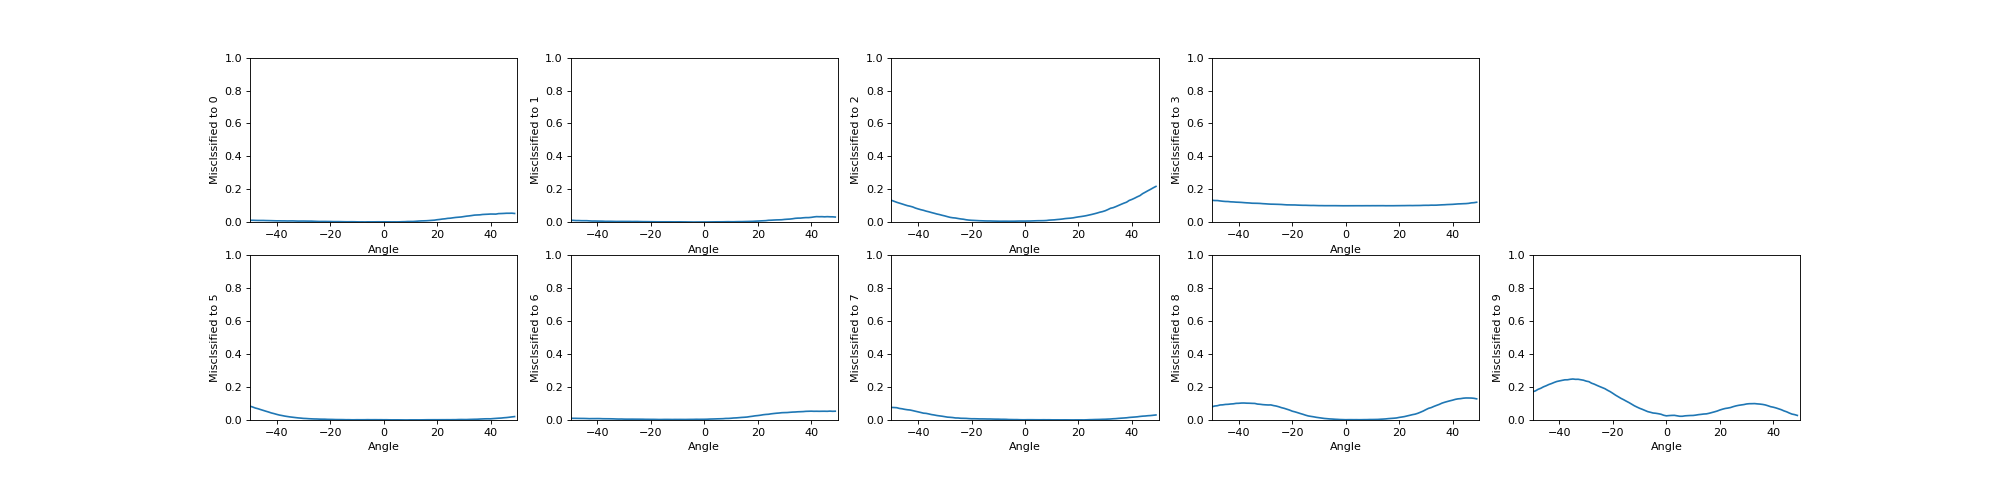
\includegraphics[width=\textwidth]{chapters/results/CNN/Rotate/acc5.png}
        \caption{Misclassification of Digit 4}
        \label{fig:Rotate-misclass1}
    \end{subfigure}
    \caption{Misclassification.}
    \label{fig:Rotate-misclassifications}
\end{figure}

\clearpage
\begin{figure}[htb!]
    \centering
    \begin{subfigure}[b]{\textwidth}
        \centering
        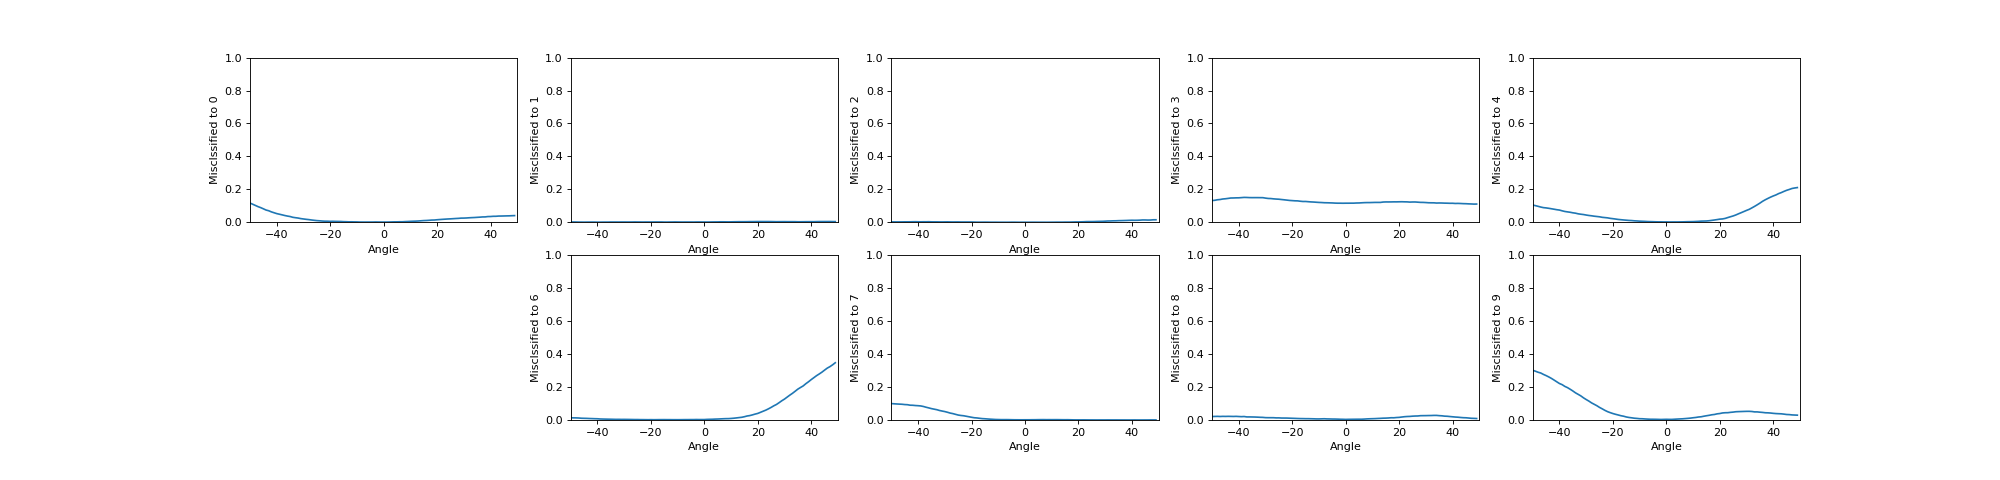
\includegraphics[width=\textwidth]{chapters/results/CNN/Rotate/acc6.png}
        \caption{Misclassification of Digit 5}
        \label{fig:Rotate-misclass0}
    \end{subfigure}
    \begin{subfigure}[b]{\textwidth}
        \centering
        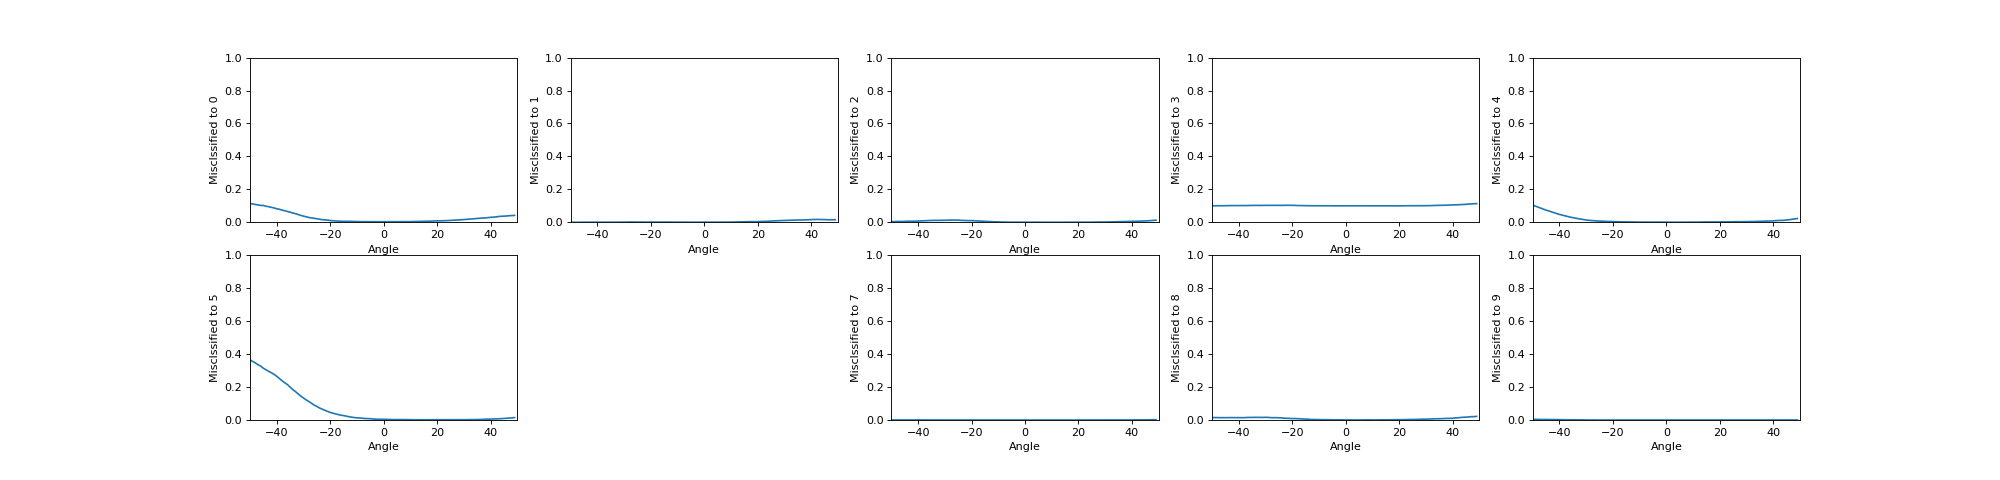
\includegraphics[width=\textwidth]{chapters/results/CNN/Rotate/acc7.png}
        \caption{Misclassification of Digit 6}
        \label{fig:Rotate-misclass0}
    \end{subfigure}
    \begin{subfigure}[b]{\textwidth}
        \centering
        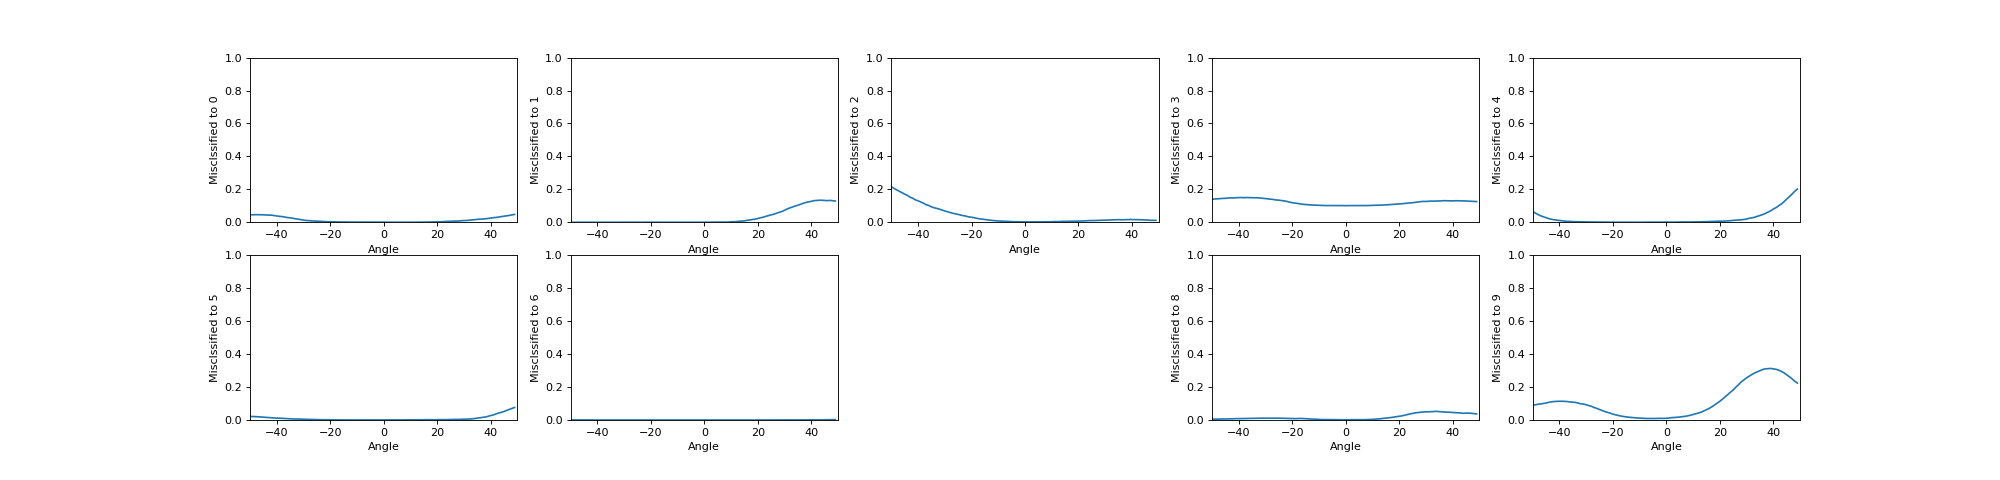
\includegraphics[width=\textwidth]{chapters/results/CNN/Rotate/acc8.png}
        \caption{Misclassification of Digit 7}
        \label{fig:Rotate-misclass0}
    \end{subfigure}
    \begin{subfigure}[b]{\textwidth}
        \centering
        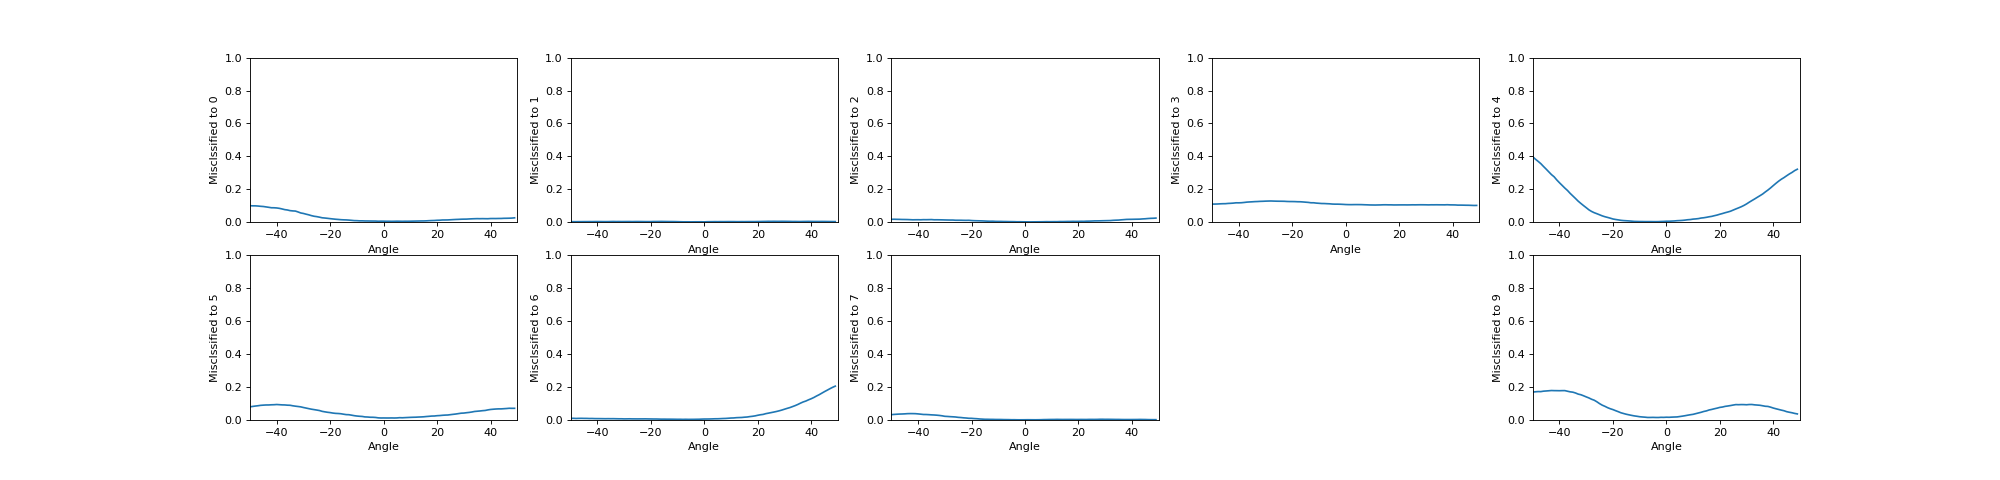
\includegraphics[width=\textwidth]{chapters/results/CNN/Rotate/acc9.png}
        \caption{Misclassification of Digit 8}
        \label{fig:Rotate-misclass0}
    \end{subfigure}
    \begin{subfigure}[b]{ \textwidth}
        \centering
        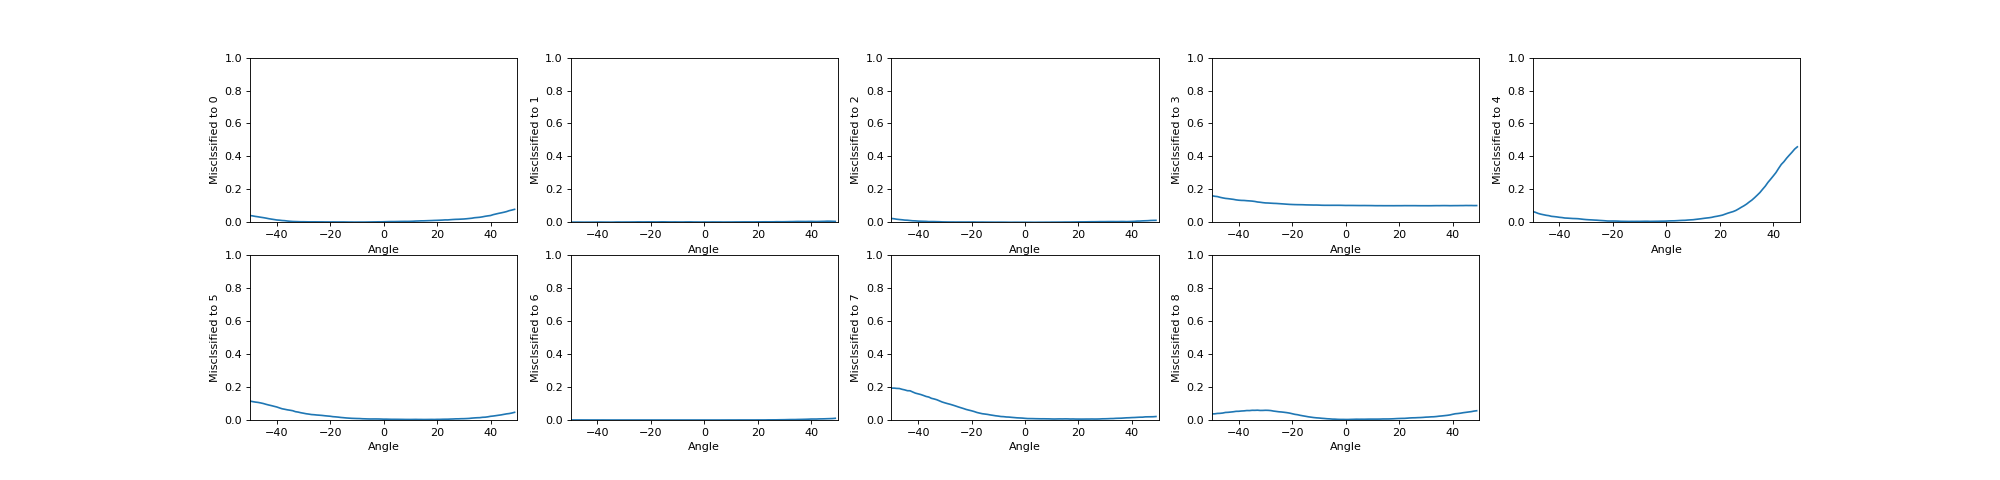
\includegraphics[width=\textwidth]{chapters/results/CNN/Rotate/acc10.png}
        \caption{Misclassification of Digit 9}
        \label{fig:Rotate-misclass1}
    \end{subfigure}
    \caption{Caption for all subfigures.}
    \label{fig:Rotate-misclassifications}
\end{figure}
        
\clearpage

\section{Overall Accuracy}
\begin{figure}[htb!]
    \centering
    \begin{subfigure}[b]{0.3\textwidth}
        \centering
        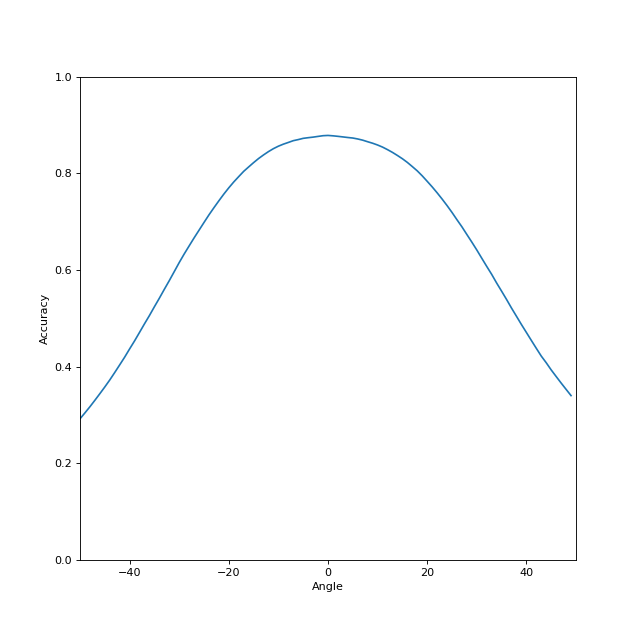
\includegraphics[width=\textwidth]{chapters/results/CNN/Rotate/acc.png}
        \caption{Rotation}
        \label{fig:Rotate-misclass0}
    \end{subfigure}
    \begin{subfigure}[b]{ 0.3\textwidth}
        \centering
        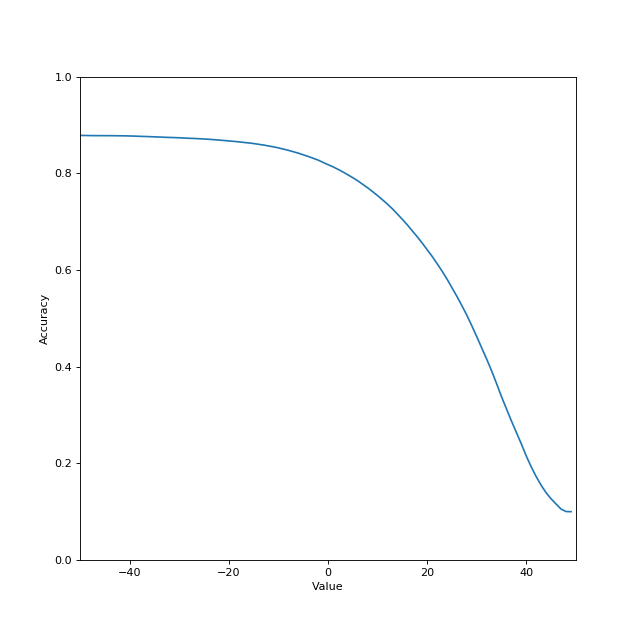
\includegraphics[width=\textwidth]{chapters/results/CNN/Shade/acc.png}
        \caption{Shading}
        \label{fig:Rotate-misclass1}
    \end{subfigure}
    \begin{subfigure}[b]{0.3\textwidth}
        \centering
        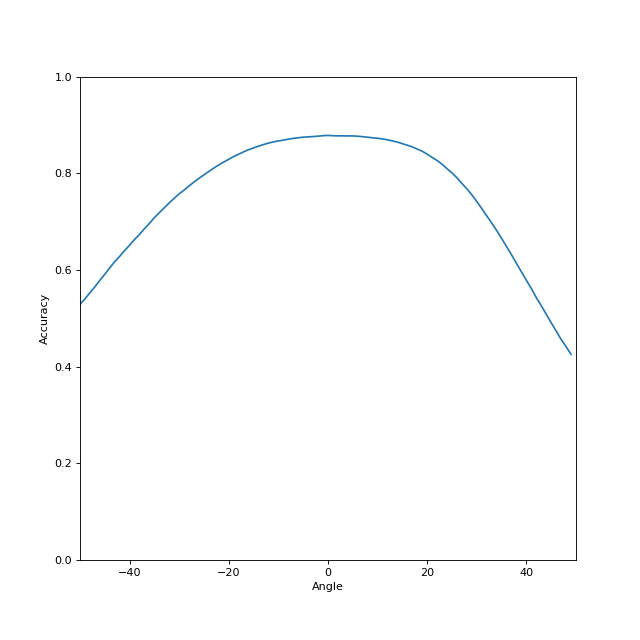
\includegraphics[width=\textwidth]{chapters/results/CNN/Shear/acc.png}
        \caption{Shearing}
        \label{fig:Rotate-misclass0}
    \end{subfigure}
    \begin{subfigure}[b]{0.3\textwidth}
        \centering
        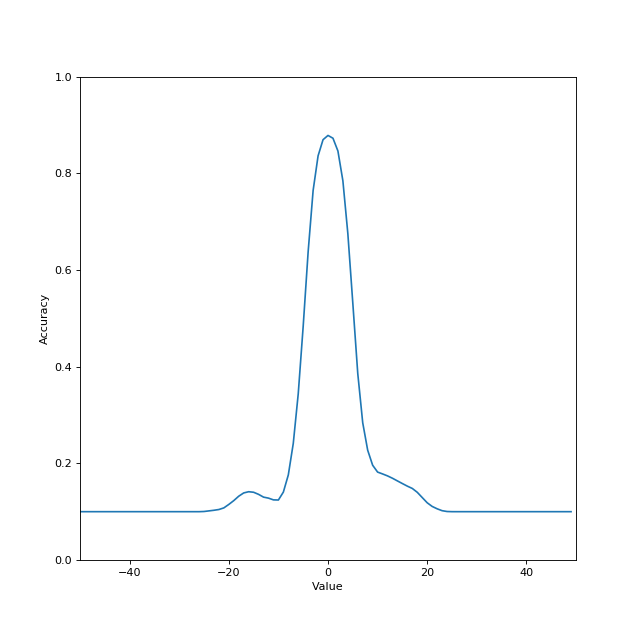
\includegraphics[width=\textwidth]{chapters/results/CNN/ShiftX/acc.png}
        \caption{Shifting in X-axis}
        \label{fig:Rotate-misclass0}
    \end{subfigure}
    \begin{subfigure}[b]{0.3\textwidth}
        \centering
        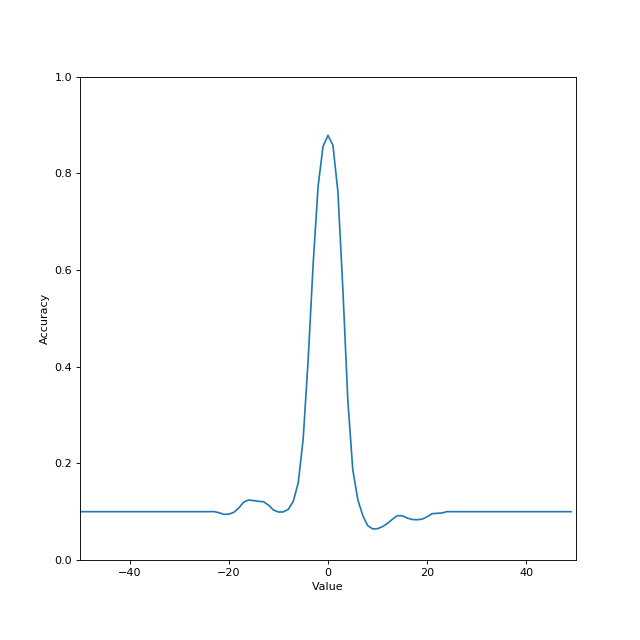
\includegraphics[width=\textwidth]{chapters/results/CNN/ShiftY/acc.png}
        \caption{Shifting in Y-axis}
        \label{fig:Rotate-misclass0}
    \end{subfigure}s
    \caption{Accuracy graphs for convolutional neural network.}
    \label{fig:Rotate-misclassifications}
\end{figure}

\clearpage
\section{Digit-by Accuracy}
\begin{figure}[htb!]
    \centering
    \begin{subfigure}[b]{\textwidth}
        \centering
        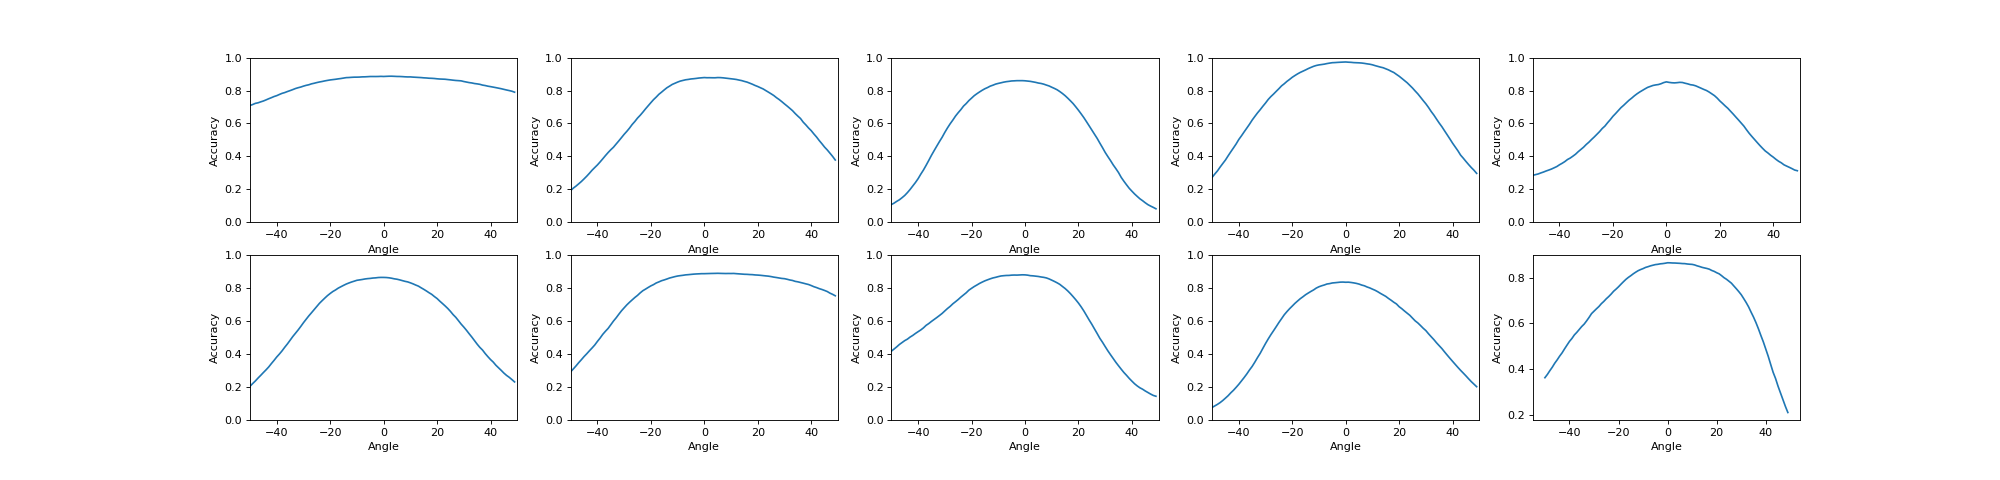
\includegraphics[width=\textwidth]{chapters/results/CNN/Rotate/accAll.png}
        \caption{Rotate}
        \label{fig:Rotate-misclass0}
    \end{subfigure}
    \begin{subfigure}[b]{\textwidth}
        \centering
        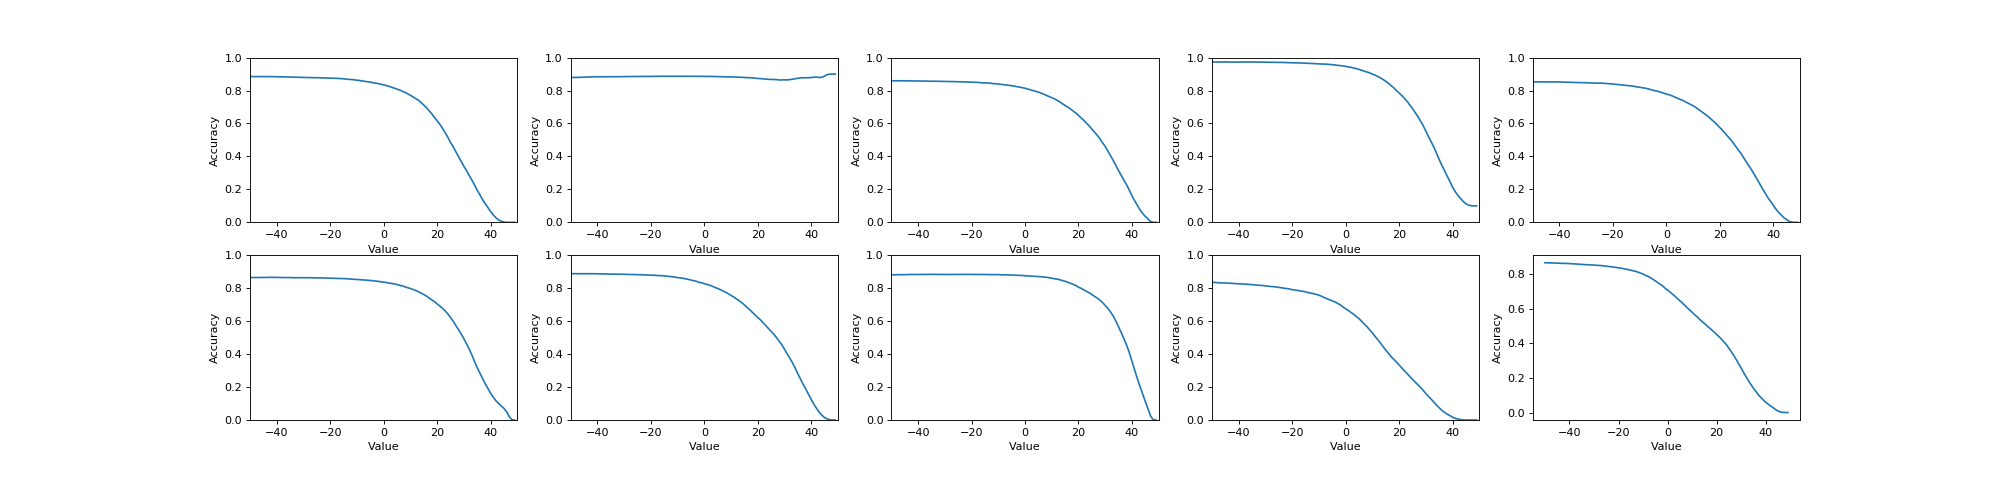
\includegraphics[width=\textwidth]{chapters/results/CNN/Shade/accAll.png}
        \caption{Shading}
        \label{fig:Rotate-misclass1}
    \end{subfigure}
    \begin{subfigure}[b]{\textwidth}
        \centering
        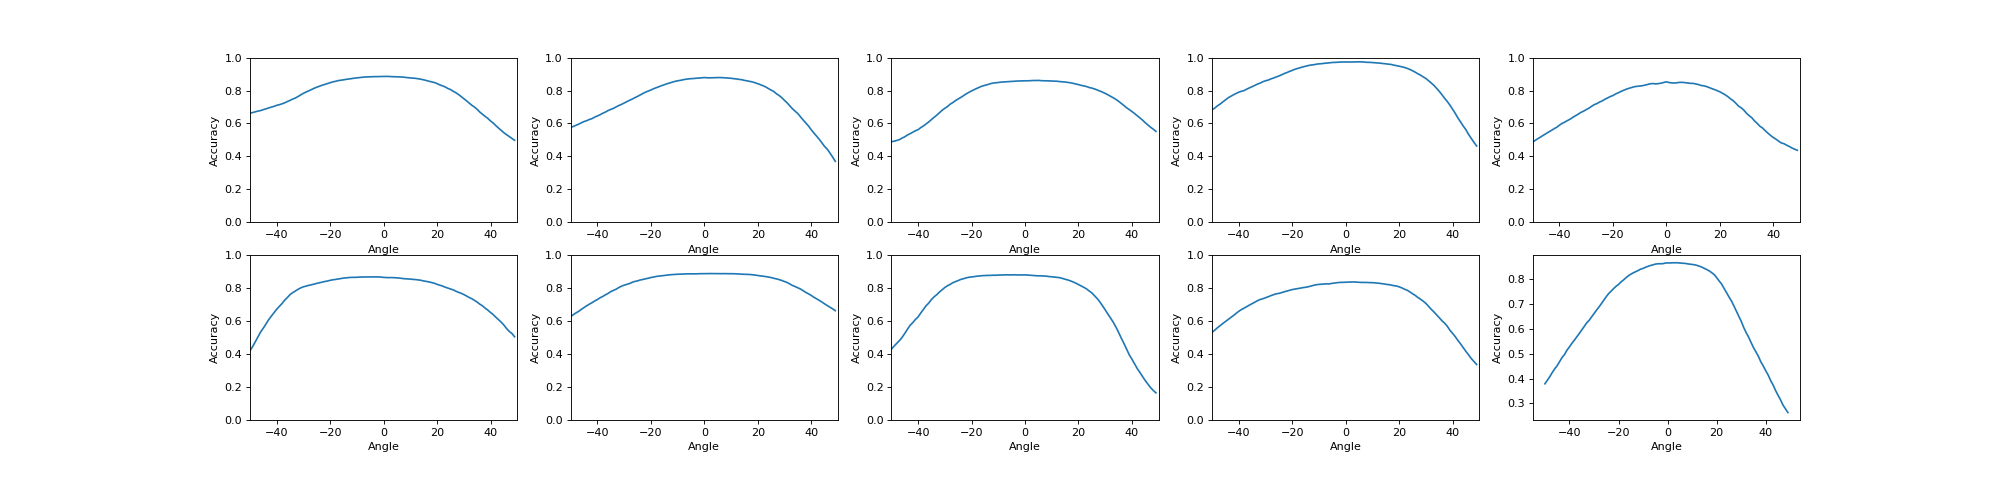
\includegraphics[width=\textwidth]{chapters/results/CNN/Shear/accAll.png}
        \caption{Shear}
        \label{fig:Rotate-misclass0}
    \end{subfigure}
    \begin{subfigure}[b]{\textwidth}
        \centering
        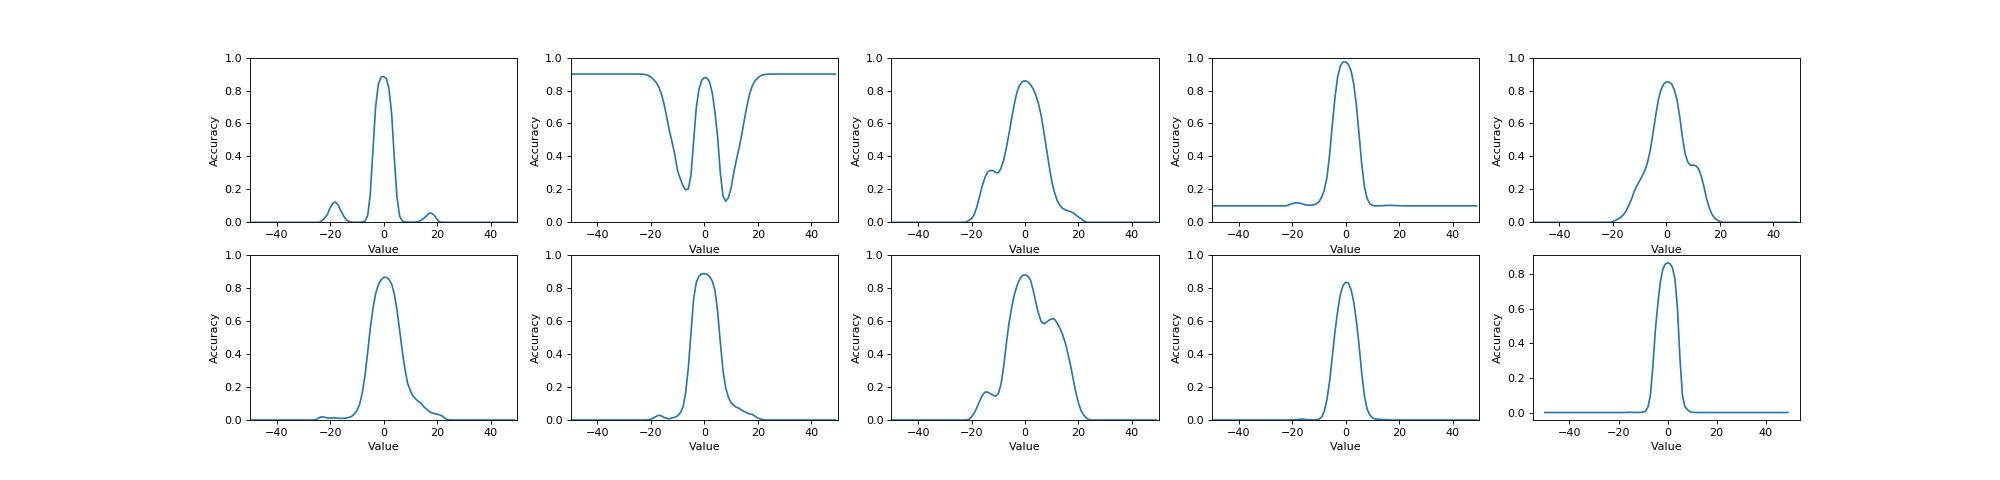
\includegraphics[width=\textwidth]{chapters/results/CNN/ShiftX/accAll.png}
        \caption{Shifting in X-axis}
        \label{fig:Rotate-misclass0}
    \end{subfigure}
    \label{fig:Rotate-misclassifications}
\end{figure}

\begin{figure}
    \centering
        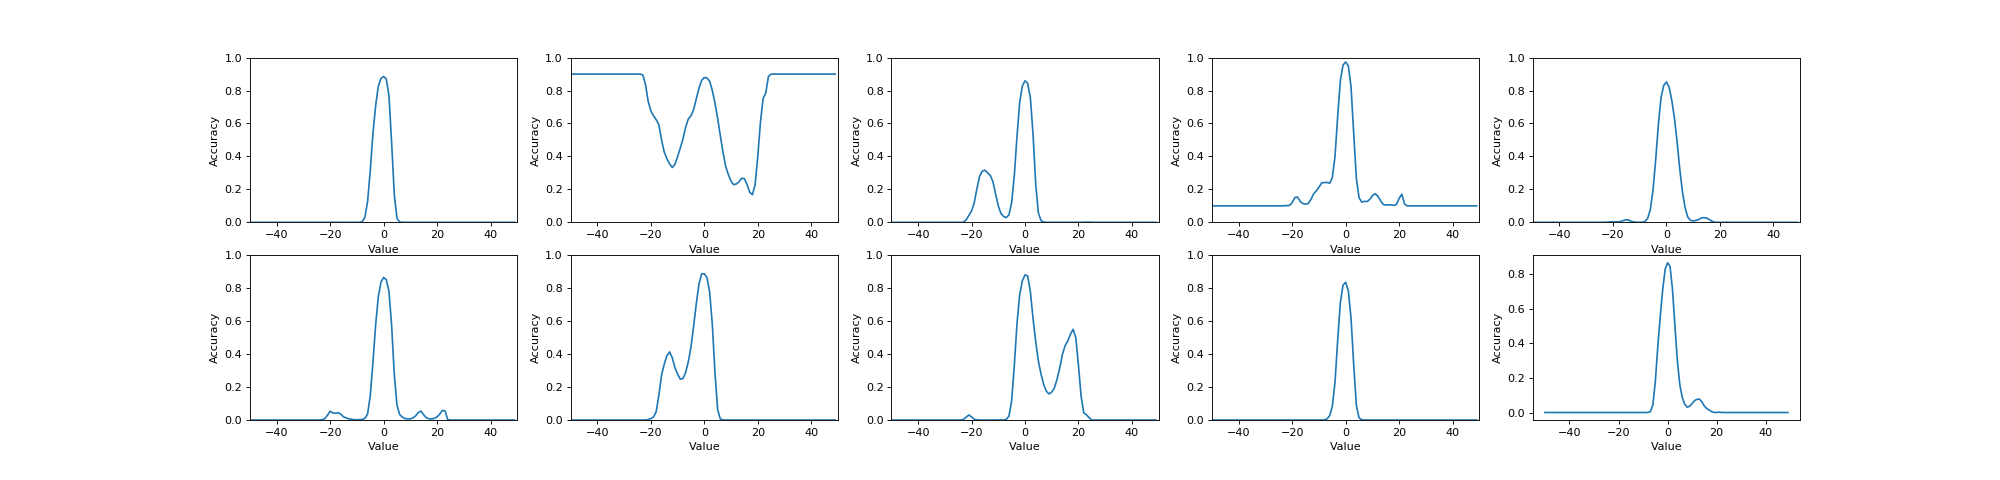
\includegraphics[width=\textwidth]{chapters/results/CNN/ShiftY/accAll.png}
        \caption{Shifting in Y-axis}
        \label{fig:Rotate-misclass0}
\end{figure}
Rotation
1.  The graph is bell shaped
2. 0 is not affected due to rotation


\iffalse
Number of instances of each digit: 1000000 \\
Confusion Matrix for rotation
Rotate
\begin{table}
\begin{tabular}{|l|l|l|l|l|l|l|l|l|l|}
\hline
935597 & 1571 & 6922 & 1439 & 12189 & 14037 & 6591 & 1488 & 9736 & 10430 \\ \hline
2156 & 681401 & 46519 & 2751 & 169826 & 27931 & 9759 & 3613 & 45566 & 10478 \\ \hline
48251 & 14436 & 625369 & 14254 & 92329 & 14828 & 21352 & 51716 & 68410 & 49055 \\ \hline
55511 & 924 & 27210 & 641320 & 49224 & 79421 & 24213 & 9285 & 45419 & 67473 \\ \hline
14679 & 7786 & 82089 & 3506 & 626526 & 22201 & 29658 & 9793 & 74675 & 129087 \\ \hline
36982 & 851 & 3881 & 20562 & 41609 & 658850 & 100751 & 8549 & 32895 & 95070 \\ \hline
14801 & 5076 & 5850 & 2183 & 21595 & 43878 & 881633 & 61 & 24041 & 882 \\ \hline
19761 & 41054 & 89028 & 12815 & 37202 & 7157 & 1548 & 604877 & 25560 & 160998 \\ \hline
44287 & 3357 & 18687 & 7605 & 99678 & 27689 & 47153 & 8077 & 664412 & 79055 \\ \hline
19214 & 3572 & 22930 & 7800 & 64705 & 32264 & 3295 & 26788 & 34992 & 784440 \\ \hline
\end{tabular}
\end{table}

Shade
\begin{table}
\begin{tabular}{|l|l|l|l|l|l|l|l|l|l|}
\hline
723812 & 170554 & 42780 & 6728 & 9156 & 22649 & 14219 & 4105 & 1688 & 4309 \\ \hline
254 & 962044 & 2730 & 390 & 2949 & 583 & 28386 & 869 & 1590 & 205 \\ \hline
5878 & 186546 & 756806 & 7351 & 5673 & 6460 & 12743 & 9246 & 6682 & 2615 \\ \hline
7909 & 197655 & 25332 & 704395 & 3671 & 26024 & 13630 & 7059 & 7924 & 6401 \\ \hline
980 & 199247 & 17353 & 83 & 736257 & 5919 & 10603 & 1859 & 4639 & 23060 \\ \hline
1759 & 185772 & 11045 & 12420 & 13794 & 736958 & 17460 & 3035 & 6985 & 10772 \\ \hline
1724 & 187885 & 29599 & 627 & 7308 & 8158 & 762263 & 73 & 2267 & 96 \\ \hline
1038 & 230118 & 7008 & 4753 & 6887 & 4707 & 1820 & 711488 & 7578 & 24603 \\ \hline
6249 & 220252 & 25119 & 7814 & 19723 & 37098 & 17413 & 4407 & 644767 & 17158 \\ \hline
3420 & 216638 & 6303 & 1732 & 48951 & 9704 & 3905 & 25036 & 11315 & 672996 \\ \hline
\end{tabular}
\end{table}

 Shear
\begin{table}
\begin{tabular}{|l|l|l|l|l|l|l|l|l|l|}
\hline
843745 & 10901 & 25910 & 6041 & 22737 & 31418 & 18795 & 6279 & 25431 & 8743 \\ \hline
489 & 827503 & 75423 & 1064 & 42026 & 5999 & 4750 & 4074 & 35602 & 3070 \\ \hline
5078 & 18985 & 841933 & 16944 & 20220 & 8561 & 24028 & 14614 & 45286 & 4351 \\ \hline
9944 & 9350 & 32310 & 764503 & 48583 & 73988 & 13401 & 4440 & 28001 & 15480 \\ \hline
9834 & 5379 & 38067 & 1622 & 780726 & 4660 & 19143 & 3798 & 28973 & 107798 \\ \hline
6990 & 7222 & 17568 & 15686 & 38861 & 840605 & 17008 & 1864 & 24632 & 29564 \\ \hline
7975 & 4004 & 23667 & 1264 & 22961 & 18252 & 902574 & 472 & 18495 & 336 \\ \hline
1905 & 83886 & 71323 & 13684 & 28050 & 4143 & 2944 & 699486 & 29394 & 65185 \\ \hline
8266 & 24716 & 60365 & 5607 & 47917 & 15477 & 21918 & 8603 & 782538 & 24593 \\ \hline
4575 & 17714 & 27060 & 5122 & 117887 & 14337 & 1801 & 34062 & 38993 & 738449 \\ \hline
\end{tabular}
\end{table}

 ShiftX
\begin{table}
\begin{tabular}{|l|l|l|l|l|l|l|l|l|l|}
\hline
77949 & 614059 & 82304 & 114994 & 10084 & 27145 & 16921 & 37383 & 15310 & 3851 \\ \hline
18598 & 762514 & 11391 & 108735 & 21327 & 19628 & 14301 & 40521 & 1593 & 1392 \\ \hline
5413 & 596299 & 158838 & 111720 & 8599 & 65944 & 29801 & 18278 & 3585 & 1523 \\ \hline
1960 & 613767 & 48437 & 192270 & 15577 & 60280 & 19406 & 37799 & 8608 & 1896 \\ \hline
10748 & 606441 & 25128 & 115124 & 143172 & 26096 & 9445 & 52487 & 2675 & 8684 \\ \hline
3280 & 576218 & 57996 & 123105 & 7793 & 122565 & 13449 & 83188 & 7653 & 4753 \\ \hline
6802 & 629739 & 79954 & 107383 & 11197 & 39254 & 112765 & 9497 & 1752 & 1657 \\ \hline
4431 & 612470 & 14042 & 104293 & 6656 & 54982 & 3929 & 188195 & 3754 & 7248 \\ \hline
11402 & 604142 & 33747 & 119427 & 14964 & 36848 & 10922 & 73575 & 84225 & 10748 \\ \hline
6458 & 610597 & 17436 & 112603 & 24052 & 23167 & 3885 & 108416 & 9620 & 83766 \\ \hline
\end{tabular}
\end{table}

 ShiftY
\begin{table}
\begin{tabular}{|l|l|l|l|l|l|l|l|l|l|}
\hline
66197 & 542587 & 43176 & 106135 & 42382 & 12674 & 70021 & 78999 & 1631 & 36198 \\ \hline
538 & 725379 & 4939 & 111517 & 12744 & 23113 & 33750 & 63499 & 898 & 23623 \\ \hline
5931 & 549369 & 84027 & 122009 & 46036 & 29879 & 50616 & 84857 & 1755 & 25521 \\ \hline
5459 & 536243 & 48175 & 173095 & 19257 & 21261 & 57625 & 90112 & 1912 & 46861 \\ \hline
5912 & 587840 & 31183 & 111527 & 72612 & 18906 & 56932 & 95170 & 958 & 18960 \\ \hline
4400 & 549322 & 56501 & 108096 & 14913 & 68901 & 55441 & 99507 & 4262 & 38657 \\ \hline
4196 & 569875 & 38726 & 108298 & 22672 & 11800 & 106513 & 75694 & 1169 & 61057 \\ \hline
6315 & 586659 & 32610 & 115134 & 43765 & 29717 & 47371 & 119460 & 1436 & 17533 \\ \hline
15388 & 533073 & 30139 & 108200 & 16740 & 19676 & 83688 & 80939 & 50348 & 61809 \\ \hline
13355 & 566917 & 27002 & 109136 & 20624 & 17805 & 81323 & 95899 & 1001 & 66938 \\ \hline
\end{tabular}
\end{table}     

\fi

\clearpage

To generate new data from MNIST digit dataset. While using rotation 0 should be in a prticular range. 1 should be in particular range.....